\documentclass[aspectratio=169,10pt]{beamer}

% Required packages
\usepackage[utf8]{inputenc}
\usepackage[T1]{fontenc}
\usepackage{amsmath,amssymb,amsthm}
\usepackage{graphicx}
\usepackage{listings}
\usepackage{xcolor}
\usepackage{tikz}
\usetikzlibrary{arrows.meta,calc}
\usepackage{algorithm}
\usepackage{algorithmic}
\usepackage{hyperref}
\usepackage{mimic}

% Theme settings
\usetheme{Madrid}
\usecolortheme{seahorse}
\setbeamertemplate{navigation symbols}{}
\setbeamertemplate{footline}[frame number]

% Code listing configuration
\lstset{
    language=Python,
    basicstyle=\ttfamily\scriptsize,
    keywordstyle=\color{blue}\bfseries,
    stringstyle=\color{red},
    commentstyle=\color{green!60!black},
    showstringspaces=false,
    breaklines=true,
    breakatwhitespace=true,
    frame=single,
    numbers=left,
    numberstyle=\tiny\color{gray},
    xleftmargin=1em,
    framexleftmargin=1em
}

% TikZ libraries
\usetikzlibrary{positioning,shapes,arrows}

% Title page information
\title{Reinforcement Learning}
\subtitle{Lecture 3: The World of Reinforcement Learning}
\author{Taehoon Kim}
\institute{Sogang University MIMIC Lab \\ \url{https://mimic-lab.com}}
\date{Fall Semester 2025}

\begin{document}

%% Slide 1: Title Page
\begin{frame}[plain]
    \titlepage
\end{frame}

%% Slide 3: Learning Objectives
\begin{frame}{Learning Objectives \& Prerequisites}

\textbf{By the end of today, you will be able to:}
\begin{itemize}
    \item Define the agent-environment interaction cycle
    \item Implement basic RL experiments with Gymnasium
    \item Calculate returns with discount factors
    \item Compare random vs heuristic policies
    \item Understand exploration-exploitation tradeoffs
    \item Create reproducible RL experiments
\end{itemize}

\vfill

\textbf{Prerequisites:}
\begin{itemize}
    \item Lecture 2: PyTorch fundamentals
    \item Python programming experience
    \item Basic probability and statistics
\end{itemize}

\end{frame}

%% Slide 4: What is Reinforcement Learning?
\begin{frame}{What is Reinforcement Learning?}

\textbf{Reinforcement Learning} is a computational approach to understanding and automating goal-directed learning and decision-making.

\vfill

\textbf{Key Characteristics:}
\begin{itemize}
    \item \textbf{Agent} learns through interaction with \textbf{environment}
    \item No supervisor, only reward signal
    \item Actions affect future observations and rewards
    \item Goal: maximize cumulative reward over time
\end{itemize}

\vfill

\textbf{Real-world Examples:}
\begin{itemize}
    \item Game playing (Chess, Go, Atari games)
    \item Robot control and navigation
    \item Resource management and scheduling
    \item Recommendation systems
\end{itemize}

\end{frame}

%% Slide 5: Agent-Environment Interface
\begin{frame}{Agent-Environment Interface}

\begin{center}
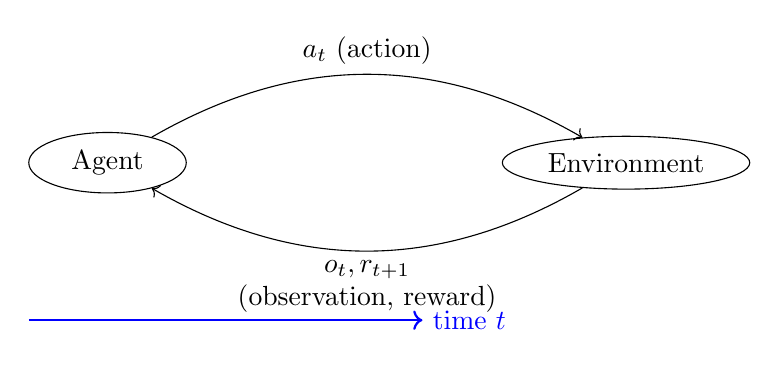
\begin{tikzpicture}[node distance=3cm, auto]
    % Nodes
    \node[draw, ellipse, minimum width=2cm] (agent) {Agent};
    \node[draw, ellipse, minimum width=2cm, right=4cm of agent] (env) {Environment};
    
    % Arrows with labels
    \draw[->] (agent) to[bend left=30] node[above] {$a_t$ (action)} (env);
    \draw[->] (env) to[bend left=30] node[below, align=center] {$o_t, r_{t+1}$\\(observation, reward)} (agent);
    
    % Time arrow
    \draw[->, thick, blue] (-1, -2) -- (4, -2) node[right] {time $t$};
\end{tikzpicture}
\end{center}

\vfill

\textbf{At each time step $t$:}
\begin{enumerate}
    \item Agent observes state/observation $o_t \in \mathcal{O}$
    \item Agent selects action $a_t \in \mathcal{A}$ using policy $\pi(a|o)$
    \item Environment transitions to new state $s_{t+1}$
    \item Agent receives reward $r_{t+1} \in \mathbb{R}$
\end{enumerate}

\end{frame}

%% Slide 6: States vs Observations
\begin{frame}{States vs Observations}

\textbf{Important Distinction:}

\vfill

\begin{columns}[t]
\column{0.48\textwidth}
\textbf{State ($s_t$):}
\begin{itemize}
    \item Complete information about environment
    \item Markov property: future depends only on current state
    \item Not always directly observable
    \item Mathematical idealization
\end{itemize}

\column{0.48\textwidth}
\textbf{Observation ($o_t$):}
\begin{itemize}
    \item What the agent actually sees
    \item May be partial or noisy
    \item Practical measurement
    \item What we work with in code
\end{itemize}
\end{columns}

\vfill

\textbf{In CartPole:}
\begin{itemize}
    \item State $\approx$ Observation: $[x, \dot{x}, \theta, \dot{\theta}]$
    \item Fully observable environment
    \item 4-dimensional continuous space
\end{itemize}

\end{frame}

%% Slide 7: Action Spaces
\begin{frame}{Action Spaces}

\textbf{Types of Action Spaces:}

\vfill

\begin{columns}[t]
\column{0.48\textwidth}
\textbf{Discrete Actions:}
\begin{itemize}
    \item Finite set of choices
    \item $\mathcal{A} = \{a_1, a_2, \ldots, a_n\}$
    \item Examples: Move left/right, buy/sell/hold
    \item CartPole: $\{0, 1\}$ (left, right)
\end{itemize}

\column{0.48\textwidth}
\textbf{Continuous Actions:}
\begin{itemize}
    \item Real-valued vectors
    \item $\mathcal{A} \subseteq \mathbb{R}^d$
    \item Examples: steering angle, force magnitude
    \item Often bounded: $[-1, 1]$
\end{itemize}
\end{columns}

\vfill

\textbf{In Gymnasium:}

\texttt{env = gym.make("CartPole-v1")}

\texttt{print(env.action\_space)  \# Discrete(2)}

\texttt{print(env.observation\_space)  \# Box(4,)}

\end{frame}

%% Slide 8: The Episode Concept
\begin{frame}[fragile]{The Episode Concept}

\textbf{Episode:} A complete sequence of agent-environment interaction from start to finish.

\vfill

\begin{center}
\textbf{Episode Timeline:}

$s_0 \xrightarrow{a_0, r_1} s_1 \xrightarrow{a_1, r_2} s_2 \xrightarrow{a_2, r_3} s_3 \rightarrow \text{Terminal}$

\vspace{0.5cm}
\textit{Observations:} $o_0, o_1, o_2, o_3$
\end{center}

\vfill

\textbf{Episode Termination:}
\begin{itemize}
    \item \textbf{Terminated:} Task completed or failed (pole falls)
    \item \textbf{Truncated:} Time limit reached (500 steps in CartPole)
    \item \textbf{Episode Length:} Number of steps taken
\end{itemize}

\vfill

\textbf{Gymnasium API:}
\begin{lstlisting}[language=Python]
obs, reward, terminated, truncated, info = env.step(action)
done = terminated or truncated
\end{lstlisting}

\end{frame}

%% Slide 9: Rewards and Returns
\begin{frame}{Rewards and Returns}

\textbf{Reward:} Immediate feedback from environment
\begin{itemize}
    \item $r_{t+1}$: reward received after taking action $a_t$
    \item Can be positive, negative, or zero
    \item CartPole: $r = +1$ for each step pole stays up
\end{itemize}

\vfill

\textbf{Return:} Cumulative reward over time
$$G_t = \sum_{k=0}^{T-t-1} r_{t+k+1}$$

\textbf{Problem:} Infinite episodes or delayed rewards

\vfill

\textbf{Discounted Return:} Weight recent rewards more
$$G_t = \sum_{k=0}^{T-t-1} \gamma^k r_{t+k+1}$$

where $\gamma \in [0,1]$ is the \textbf{discount factor}

\end{frame}

%% Slide 10: Understanding the Discount Factor
\begin{frame}{Understanding the Discount Factor}

\begin{columns}[t]
\column{0.48\textwidth}
\textbf{$\gamma = 0$ (Myopic):}
\begin{itemize}
    \item Only immediate reward matters
    \item $G_t = r_{t+1}$
    \item Very short-term thinking
\end{itemize}

\vfill

\textbf{$\gamma = 1$ (Farsighted):}
\begin{itemize}
    \item All future rewards matter
    \item $G_t = \sum r_{t+k+1}$
    \item May not converge
\end{itemize}

\column{0.48\textwidth}
\textbf{$\gamma \in (0,1)$ (Balanced):}
\begin{itemize}
    \item Near rewards > distant rewards
    \item Common values: 0.9, 0.95, 0.99
    \item Ensures convergence
\end{itemize}

\vfill

\textbf{Example ($\gamma = 0.9$):}
\begin{align}
G_0 &= r_1 + 0.9 r_2 + 0.81 r_3 + \ldots\\
&= 1 + 0.9 + 0.81 + 0.729 + \ldots
\end{align}
\end{columns}

\end{frame}

%% Slide 11: Policy Definition
\begin{frame}{Policy Definition}

\textbf{Policy ($\pi$):} A strategy for selecting actions

\vfill

\textbf{Deterministic Policy:}
$$\pi(s) = a$$
\begin{itemize}
    \item Always selects same action for same state
    \item Simple but limited exploration
\end{itemize}

\vfill

\textbf{Stochastic Policy:}
$$\pi(a|s) = P(\text{select action } a \text{ in state } s)$$
\begin{itemize}
    \item Probability distribution over actions
    \item Enables exploration and uncertainty handling
    \item $\sum_a \pi(a|s) = 1$ for all $s$
\end{itemize}

\end{frame}

%% Slide 12: The Exploration-Exploitation Dilemma
\begin{frame}{The Exploration-Exploitation Dilemma}

\textbf{Core Challenge in RL:}

\vfill

\begin{columns}[t]
\column{0.48\textwidth}
\textbf{Exploitation:}
\begin{itemize}
    \item Choose best known action
    \item Maximize immediate reward
    \item Risk: missing better options
    \item "Greedy" behavior
\end{itemize}

\column{0.48\textwidth}
\textbf{Exploration:}
\begin{itemize}
    \item Try unknown actions
    \item Gather new information
    \item Risk: lower immediate reward
    \item "Curious" behavior
\end{itemize}
\end{columns}

\vfill

\textbf{Real-world Analogy:}
\begin{itemize}
    \item Restaurant choice: favorite (exploit) vs new place (explore)
    \item Investment: safe bonds (exploit) vs risky stocks (explore)
    \item Route to work: known path vs trying shortcuts
\end{itemize}

\vfill

\textcolor{red}{\textbf{Key Insight:}} Need both for optimal long-term performance!

\end{frame}

%% Slide 13: Epsilon-Greedy Strategy
\begin{frame}{$\varepsilon$-Greedy Strategy}

\textbf{Simple Solution to Exploration-Exploitation:}

\vfill

$$\pi_{\varepsilon}(a|s) = \begin{cases}
1 - \varepsilon + \frac{\varepsilon}{|\mathcal{A}|} & \text{if } a = \arg\max_a Q(s,a) \\
\frac{\varepsilon}{|\mathcal{A}|} & \text{otherwise}
\end{cases}$$

\vfill

\textbf{In Simple Terms:}
\begin{itemize}
    \item With probability $(1-\varepsilon)$: choose best action (exploit)
    \item With probability $\varepsilon$: choose random action (explore)
    \item $\varepsilon \in [0,1]$ controls exploration amount
\end{itemize}

\vfill

\textbf{Common Values:}
\begin{itemize}
    \item $\varepsilon = 0.1$: 90\% exploitation, 10\% exploration
    \item $\varepsilon = 0.01$: 99\% exploitation, 1\% exploration
    \item Often decayed over time: high exploration $\rightarrow$ low exploration
\end{itemize}

\end{frame}

%% Slide 14: CartPole Environment Details
\begin{frame}{CartPole Environment Details}

\begin{columns}[T]  % 위쪽 정렬
  % ---------- 왼쪽: 텍스트 ----------
  \begin{column}{0.4\textwidth}

  \textbf{State Variables:}
  \begin{itemize}
      \item $x$: cart position on track
      \item $\dot{x}$: cart velocity
      \item $\theta$: pole angle from vertical
      \item $\dot{\theta}$: angular velocity of pole
  \end{itemize}

  \vfill

  \textbf{Actions:}
  \begin{itemize}
      \item 0: Push cart left
      \item 1: Push cart right
  \end{itemize}

  \vfill

  \textbf{Termination Conditions:}
  \begin{itemize}
      \item Pole angle $> 12^\circ$ from vertical
      \item Cart position $> 2.4$ units from center
      \item Episode length $> 500$ steps (truncation)
  \end{itemize}

  \end{column}

\begin{column}{0.6\textwidth}
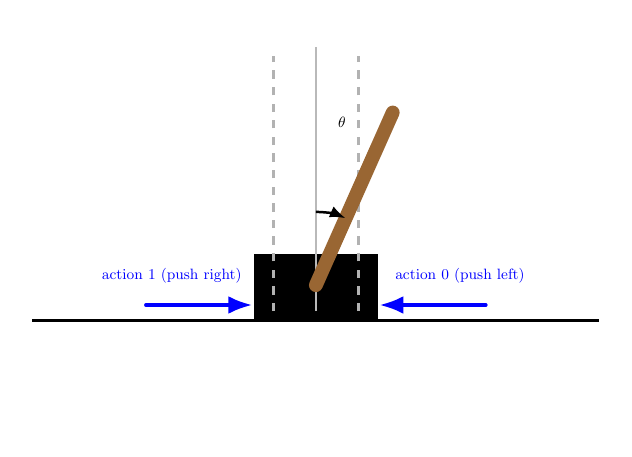
\begin{tikzpicture}[
    x=1cm, y=1cm, scale=0.6, transform shape, >=Latex,
    force/.style={-{Latex[length=3mm]}, very thick, blue, line cap=round},
    ref/.style={dash pattern=on 3pt off 3pt, line width=0.9pt, gray!60},
    note/.style={font=\small}
]

% 컬럼 밖 넘침 방지
\path[use as bounding box] (-6.1,-2.3) rectangle (6.1,6.2);

% 트랙
\draw[line width=1.3pt] (-6,0) -- (6,0);

% 카트와 축
\def\cartW{2.6}
\def\cartH{1.4}
\coordinate (C) at (0,0.75);
\draw[fill=black] (-\cartW/2,0) rectangle (\cartW/2,\cartH);
\fill[gray!70] (C) circle (2pt);

% 수직 기준선들
\draw[ref] (-0.9,0.2) -- (-0.9,5.6);
\draw[gray!55,line width=0.6pt] (0,0.2) -- (0,5.8);  % 중앙 얇은 실선
\draw[ref] (0.9,0.2) -- (0.9,5.6);

% 폴: 수직에서 우측으로 ang만큼 기울임
\def\ang{24}     % 수직 대비 양의 각도(오른쪽)
\def\L{4.0}      % 폴 길이
\draw[line width=5pt, brown!80!black, line cap=round]
      (C) -- ($(C)+(90-\ang:\L)$);

% θ: 수직선과 폴 사이의 각. 시계방향 호를 'delta angle'로 확정
\draw[-{Latex[length=2mm]}, line width=0.9pt]
      (C) ++(0,1.55) [shift={(C)}]
      arc[start angle=90, delta angle=-\ang, radius=1.55];
\node[note] at ($(C)+(0.55,3.45)$) {$\theta$};


% 액션 화살표와 라벨(텍스트는 위로, 화살표는 트랙 바로 위)
\draw[force] (-3.6,0.33) -- (-1.35,0.33);
\draw[force] ( 3.6,0.33) -- ( 1.35,0.33);
\node[note, blue] at (-3.05,0.95) {action 1 (push right)};
\node[note, blue] at ( 3.05,0.95) {action 0 (push left)};


\end{tikzpicture}
\end{column}
\end{columns}

\end{frame}

%% Slide 15: CartPole Heuristic Policy
\begin{frame}[fragile]{CartPole Heuristic Policy}

\textbf{Simple Control Strategy:}

\begin{lstlisting}
def heuristic_policy(obs):
    """Push cart toward direction that stabilizes pole"""
    x, x_dot, theta, theta_dot = obs
    
    # Combined signal: angle + angular velocity
    control_signal = theta + 0.5 * theta_dot
    
    # Push right if pole leaning/falling right
    return 1 if control_signal > 0.0 else 0
\end{lstlisting}

\vfill

\textbf{Intuition:}
\begin{itemize}
    \item $\theta > 0$: pole leaning right $\rightarrow$ push cart right
    \item $\theta < 0$: pole leaning left $\rightarrow$ push cart left  
    \item $\dot{\theta}$: anticipate future lean direction
    \item Not optimal, but much better than random!
\end{itemize}

\end{frame}

%% Slide 16: Implementing Epsilon-Greedy
\begin{frame}[fragile]{Implementing $\varepsilon$-Greedy}

\begin{lstlisting}
def create_epsilon_greedy_policy(base_policy, epsilon=0.1):
    """Create epsilon-greedy version of any policy"""
    def epsilon_greedy_policy(obs):
        if np.random.random() < epsilon:
            # Explore: random action
            return np.random.randint(0, 2)  # CartPole actions
        else:
            # Exploit: use base policy
            return base_policy(obs)
    
    return epsilon_greedy_policy

# Usage
heuristic_eps = create_epsilon_greedy_policy(
    heuristic_policy, epsilon=0.1
)
\end{lstlisting}

\vfill

\textbf{Benefits:}
\begin{itemize}
    \item Wraps any deterministic policy
    \item Controlled randomness for exploration
    \item Still mostly follows good decisions
\end{itemize}

\end{frame}

%% Slide 17: Standard Code Header Review
\begin{frame}[fragile]{Standard Code Header Review}

\textbf{Reproducibility Setup:}

\begin{lstlisting}
# PyTorch 2.x Standard Practice Header
import os, random, numpy as np, torch

def setup_seed(seed=42):
    random.seed(seed)
    np.random.seed(seed)  
    torch.manual_seed(seed)
    if torch.cuda.is_available():
        torch.cuda.manual_seed_all(seed)

# Proper device selection (CUDA > MPS > CPU)
device = torch.device(
    'cuda' if torch.cuda.is_available() 
    else 'mps' if hasattr(torch.backends, 'mps') and torch.backends.mps.is_available()
    else 'cpu'
)
amp_enabled = torch.cuda.is_available()
setup_seed(42)
\end{lstlisting}

\textbf{Key Points:} All random sources seeded, device auto-selection

\end{frame}

%% Slide 18: Environment Creation Utility
\begin{frame}[fragile]{Environment Creation Utility}

\begin{lstlisting}
import gymnasium as gym

def make_env(env_id="CartPole-v1", seed=42):
    """Create properly seeded environment"""
    env = gym.make(env_id)
    env.reset(seed=seed)
    env.action_space.seed(seed)
    env.observation_space.seed(seed)
    return env

# Usage
env = make_env("CartPole-v1", seed=42)
obs, info = env.reset()  # obs shape: (4,)

print(f"Observation: {obs}")
print(f"Action space: {env.action_space}")  # Discrete(2)
print(f"Obs space: {env.observation_space}")  # Box(4,)
\end{lstlisting}

\vfill

\textbf{Important:} Seed environment AND its spaces for full reproducibility

\end{frame}

%% Slide 19: Episode Collection Function
\begin{frame}[fragile,shrink=6]{Episode Collection Function}

\begin{lstlisting}
def collect_episode(env, policy, max_steps=500):
    """Collect one episode using given policy"""
    obs, info = env.reset()
    
    episode_data = {
        'observations': [obs.copy()],
        'actions': [],
        'rewards': [],
        'terminated': False,
        'truncated': False
    }
    
    for step in range(max_steps):
        action = policy(obs)
        episode_data['actions'].append(action)
        
        obs, reward, terminated, truncated, info = env.step(action)
        episode_data['rewards'].append(reward)
        episode_data['observations'].append(obs.copy())
        
        if terminated or truncated:
            episode_data['terminated'] = terminated
            episode_data['truncated'] = truncated
            break
    
    return episode_data
\end{lstlisting}

\end{frame}

%% Slide 20: Return Calculation
\begin{frame}[fragile]{Return Calculation}

\begin{lstlisting}
def calculate_returns(rewards, gamma=0.99):
    """Calculate discounted returns from reward sequence"""
    returns = []
    G = 0.0
    
    # Work backwards through episode
    for reward in reversed(rewards):
        G = reward + gamma * G
        returns.append(G)
    
    # Reverse to get forward-time order
    return list(reversed(returns))

# Example
rewards = [1.0, 1.0, 1.0, 1.0, 1.0]  # 5 steps
returns_09 = calculate_returns(rewards, gamma=0.9)
returns_099 = calculate_returns(rewards, gamma=0.99)

print(f"gamma=0.9:  G_0 = {returns_09[0]:.3f}")   # ~4.095
print(f"gamma=0.99: G_0 = {returns_099[0]:.3f}")  # ~4.901
\end{lstlisting}

\textbf{Higher $\gamma$} $\rightarrow$ higher returns (values future more)

\end{frame}

%% Slide 21: Policy Evaluation Function
\begin{frame}[fragile]{Policy Evaluation Function}

\begin{lstlisting}
def evaluate_policy(env_id, policy, episodes=10, seed=123):
    """Evaluate policy performance over multiple episodes"""
    env = make_env(env_id, seed=seed)
    returns = []
    
    for episode in range(episodes):
        # Different seed per episode for variety
        env.reset(seed=seed + episode)
        
        obs, _ = env.reset()
        total_reward = 0.0
        
        while True:
            action = policy(obs)
            obs, reward, terminated, truncated, _ = env.step(action)
            total_reward += reward
            
            if terminated or truncated:
                break
        
        returns.append(total_reward)
    
    env.close()
    return np.array(returns)
\end{lstlisting}

\end{frame}

%% Slide 22: TensorBoard Logging
\begin{frame}[fragile]{TensorBoard Logging}

\begin{lstlisting}
from torch.utils.tensorboard import SummaryWriter

def log_experiment_results(policy_results, logdir="runs/lecture3"):
    """Log policy comparison results to TensorBoard"""
    writer = SummaryWriter(log_dir=logdir)
    
    for policy_name, returns in policy_results.items():
        for episode, return_val in enumerate(returns):
            writer.add_scalar(
                f"EpisodeReturn/{policy_name}", 
                return_val, 
                episode
            )
        
        # Summary statistics
        writer.add_scalar(f"MeanReturn/{policy_name}", 
                         np.mean(returns), 0)
        writer.add_histogram(f"ReturnDistribution/{policy_name}",
                           returns, 0)
    
    writer.close()
    print(f"Results logged to {logdir}")
    print("View with: tensorboard --logdir=runs/lecture3")
\end{lstlisting}

\end{frame}


%% Slide 24: Experiment Overview
\begin{frame}{Experiment Overview - Next 70 Minutes}

\textbf{9 Progressive Experiments:}

\begin{enumerate}
    \item \textbf{exp01\_setup.py} - Environment verification (5 min)
    \item \textbf{exp02\_rl\_basics.py} - Agent-environment interaction (8 min)
    \item \textbf{exp03\_returns\_discounting.py} - Return calculations (8 min)
    \item \textbf{exp04\_exploration\_exploitation.py} - Policy comparison (10 min)
    \item \textbf{exp05\_standard\_header.py} - Code organization (5 min)
    \item \textbf{exp06\_cartpole\_heuristics.py} - Heuristic policies (8 min)
    \item \textbf{exp07\_tensorboard\_logging.py} - Results visualization (8 min)
    \item \textbf{exp08\_statistical\_analysis.py} - Performance analysis (8 min)
    \item \textbf{exp09\_integrated\_test.py} - Full validation (10 min)
\end{enumerate}

\vfill

\textcolor{blue}{\textbf{Goal:}} Build complete RL experimental pipeline step by step

\end{frame}

%% Slide 25: Experiment 01 - Setup Verification
\begin{frame}[fragile]{Experiment 01: Setup Verification}

\textbf{Objective:} Verify Gymnasium installation and basic environment functionality

\begin{lstlisting}
# Run this experiment
python exp01_setup.py

# Expected outputs:
# - System configuration metadata
# - Environment creation test
# - Basic interaction test  
# - Reproducibility verification
# - "ALL TESTS PASSED" message
\end{lstlisting}

\vfill

\textbf{Key Checks:}
\begin{itemize}
    \item Gymnasium environment creation
    \item Observation/action space properties  
    \item Reset/step API correctness
    \item Seeding reproducibility
    \item Device configuration
\end{itemize}

\vfill

\textcolor{red}{\textbf{Stop here if any test fails!}} Fix issues before proceeding.

\end{frame}

%% Slide 26: Experiment 02 - RL Basics
\begin{frame}[fragile]{Experiment 02: RL Basics}

\textbf{Objective:} Understand agent-environment interaction through episode collection

\begin{lstlisting}
# Run and analyze
python exp02_rl_basics.py

# Generates:
# - 20 episodes with random policy
# - Episode statistics (length, rewards, termination)
# - Visualization plots (if matplotlib available)
# - JSON file with detailed data
\end{lstlisting}

\vfill

\textbf{Key Concepts Demonstrated:}
\begin{itemize}
    \item Episode data structure
    \item Terminated vs truncated episodes
    \item Random policy baseline performance
    \item Statistical analysis of episodes
\end{itemize}

\vfill

\textbf{Expected Results:} Random policy gets ~22 ± 20 reward on average

\end{frame}

%% Slide 27: Experiment 03 - Returns & Discounting
\begin{frame}[fragile]{Experiment 03: Returns \& Discounting}

\textbf{Objective:} Implement and understand discounted return calculations

\begin{lstlisting}
# Test different discount factors
python exp03_returns_discounting.py

# Compares gamma values: 0.0, 0.5, 0.9, 0.95, 0.99, 1.0
# Shows impact on return calculations
# Visualizes return vs episode position
\end{lstlisting}

\vfill

\textbf{Key Insights:}
\begin{itemize}
    \item $\gamma = 0$: Only immediate reward matters
    \item $\gamma = 1$: All future rewards equally important
    \item $\gamma \in (0,1)$: Balanced temporal perspective
    \item Higher $\gamma$ $\rightarrow$ higher returns for same episode
\end{itemize}

\vfill

\textbf{Mathematical Verification:} $G_t = r_{t+1} + \gamma G_{t+1}$

\end{frame}

%% Slide 28: Experiment 04 - Exploration vs Exploitation
\begin{frame}[fragile]{Experiment 04: Exploration vs Exploitation}

\textbf{Objective:} Compare different exploration strategies

\begin{lstlisting}
# Compare policies with different exploration rates
python exp04_exploration_exploitation.py

# Tests:
# - Pure random policy
# - Pure heuristic policy  
# - Epsilon-greedy with eps = [0.0, 0.1, 0.2, 0.4]
# - Statistical significance testing
\end{lstlisting}

\vfill

\textbf{Expected Ranking:}
\begin{enumerate}
    \item Pure heuristic ($\varepsilon = 0$): ~480 ± 50
    \item $\varepsilon$-greedy ($\varepsilon = 0.1$): ~430 ± 60  
    \item $\varepsilon$-greedy ($\varepsilon = 0.2$): ~380 ± 70
    \item Pure random: ~22 ± 20
\end{enumerate}

\vfill

\textcolor{blue}{\textbf{Key Finding:}} Small exploration helps in noisy environments!

\end{frame}

%% Slide 29: Experiment 05 - Standard Header
\begin{frame}[fragile]{Experiment 05: Standard Header}

\textbf{Objective:} Organize reusable code components

\begin{lstlisting}
# Validate code organization
python exp05_standard_header.py

# Tests:
# - Import functionality
# - Device selection logic
# - Seeding consistency
# - Utility function correctness
\end{lstlisting}

\vfill

\textbf{Code Organization Benefits:}
\begin{itemize}
    \item Consistent device handling across experiments
    \item Reproducible seeding setup
    \item Reusable environment utilities
    \item Cleaner experiment scripts
\end{itemize}

\vfill

\textbf{Best Practice:} Create reusable modules for common RL operations

\end{frame}

%% Slide 30: Experiment 06 - CartPole Heuristics
\begin{frame}[fragile]{Experiment 06: CartPole Heuristics}

\textbf{Objective:} Design and test domain-specific heuristic policies

\begin{lstlisting}
# Test multiple heuristic strategies
python exp06_cartpole_heuristics.py

# Heuristics tested:
# 1. Angle-only: based on theta
# 2. Angle + velocity: theta + 0.5*theta_dot  
# 3. Full state: includes cart position/velocity
# 4. Tuned coefficients
\end{lstlisting}

\vfill

\textbf{Heuristic Design Principles:}
\begin{itemize}
    \item Use domain knowledge (physics of CartPole)
    \item Combine multiple relevant state variables
    \item Test different coefficient weights
    \item Compare against random baseline
\end{itemize}

\vfill

\textbf{Engineering Insight:} Good heuristics often outperform naive RL initially

\end{frame}

%% Slide 32: Experiment 07 - TensorBoard Logging
\begin{frame}[fragile]{Experiment 07: TensorBoard Logging}

\textbf{Objective:} Learn professional experiment logging and visualization

\begin{lstlisting}
# Create comprehensive logs
python exp07_tensorboard_logging.py

# Generates:
# - Scalar metrics (returns, episode lengths)
# - Histograms (return distributions) 
# - Text logs (experiment metadata)
# - Comparative plots across policies
\end{lstlisting}

\vfill

\textbf{TensorBoard Features Used:}
\begin{itemize}
    \item \texttt{add\_scalar()}: Time series metrics
    \item \texttt{add\_histogram()}: Distribution visualization
    \item \texttt{add\_text()}: Experiment documentation
    \item Organized namespaces: \texttt{Policy/Random}, \texttt{Policy/Heuristic}
\end{itemize}

\vfill

\textbf{View Results:} \texttt{tensorboard --logdir=runs/lecture3}

\end{frame}

%% Slide 33: Experiment 08 - Statistical Analysis
\begin{frame}[fragile]{Experiment 08: Statistical Analysis}

\textbf{Objective:} Rigorous statistical comparison of policies

\begin{lstlisting}
# Statistical testing and analysis
python exp08_statistical_analysis.py

# Performs:
# - Bootstrap confidence intervals
# - Effect size calculations (Cohen's d)
# - Statistical significance testing (t-tests)
# - Power analysis for sample size
\end{lstlisting}

\vfill

\textbf{Statistical Concepts:}
\begin{itemize}
    \item \textbf{Bootstrap CI:} Non-parametric confidence intervals
    \item \textbf{Effect Size:} Practical significance beyond p-values
    \item \textbf{Sample Size:} How many episodes needed for reliable results?
    \item \textbf{Multiple Comparisons:} Bonferroni correction
\end{itemize}

\vfill

\textbf{Scientific Rigor:} Proper statistics essential for RL research

\end{frame}

%% Slide 34: Experiment 09 - Integrated Test
\begin{frame}[fragile]{Experiment 09: Integrated Test}

\textbf{Objective:} Comprehensive validation of all Lecture 3 components

\begin{lstlisting}
# Full integration test
python exp09_integrated_test.py

# Validates:
# - All previous experiments work correctly
# - End-to-end reproducibility 
# - Statistical consistency
# - Visualization generation
# - Complete experimental pipeline
\end{lstlisting}

\vfill

\textbf{Integration Tests Include:}
\begin{itemize}
    \item Environment setup verification
    \item Policy implementation correctness
    \item Return calculation accuracy
    \item Reproducibility across runs
    \item Full experimental workflow
\end{itemize}

\vfill

\textcolor{green}{\textbf{Success Criteria:}} All tests pass, ready for Lecture 4!

\end{frame}

%% Slide 35: Understanding Random Policy Results
\begin{frame}{Understanding Random Policy Results}

\textbf{What to Expect from Random Policy:}

\vfill

\textbf{Theoretical Analysis:}
\begin{itemize}
    \item Each action has 50\% probability
    \item No feedback utilization  
    \item Episode length follows geometric distribution
    \item Expected length $\approx 20-25$ steps on CartPole
\end{itemize}

\vfill

\textbf{Empirical Observations:}
\begin{itemize}
    \item High variability (some episodes very short, few longer)
    \item Most episodes terminate due to pole falling
    \item Rarely reaches 500-step truncation
    \item Performance ceiling around $\sim 30$ reward
\end{itemize}

\vfill

\textbf{Why Random Policy Matters:}
\begin{itemize}
    \item Establishes baseline performance
    \item Tests environment correctness
    \item Demonstrates need for learning
\end{itemize}

\end{frame}

%% Slide 36: Understanding Heuristic Policy Results
\begin{frame}{Understanding Heuristic Policy Results}

\textbf{What to Expect from Heuristic Policy:}

\vfill

\textbf{Performance Characteristics:}
\begin{itemize}
    \item Much better than random: ~400-500 reward
    \item Often reaches 500-step truncation
    \item Lower variability than random
    \item Occasional failures due to edge cases
\end{itemize}

\vfill

\textbf{Failure Modes:}
\begin{itemize}
    \item Extreme initial conditions (large angle/velocity)
    \item Control signal noise accumulation
    \item Lack of learning from experience
    \item Fixed coefficients not optimal
\end{itemize}

\vfill

\textbf{Educational Value:}
\begin{itemize}
    \item Shows power of domain knowledge
    \item Demonstrates exploration vs exploitation
    \item Baseline for learning algorithms
\end{itemize}

\end{frame}

%% Slide 37: Epsilon-Greedy Trade-offs
\begin{frame}{$\varepsilon$-Greedy Trade-offs}

\textbf{Performance vs Exploration Level:}

\begin{center}
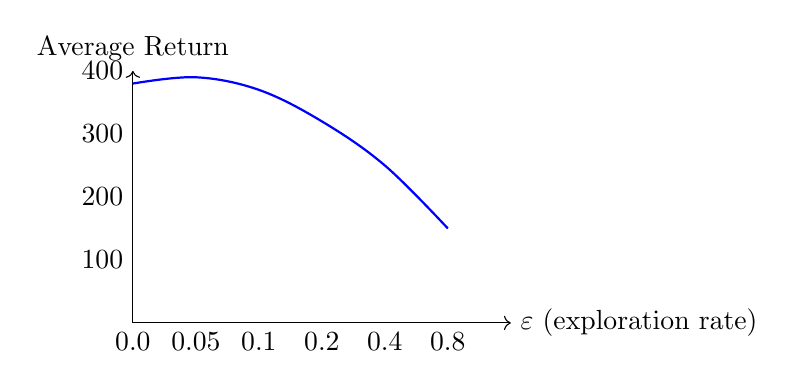
\begin{tikzpicture}[scale=0.8]
    \draw[->] (0,0) -- (6,0) node[right] {$\varepsilon$ (exploration rate)};
    \draw[->] (0,0) -- (0,4) node[above] {Average Return};
    
    % Performance curve (inverted U shape)
    \draw[thick, blue] plot[smooth, tension=0.6] coordinates {
        (0,3.8) (1,3.9) (2,3.7) (3,3.2) (4,2.5) (5,1.5)
    };
    
    % Labels
    \node[below] at (0,0) {0.0};
    \node[below] at (1,0) {0.05};
    \node[below] at (2,0) {0.1};
    \node[below] at (3,0) {0.2};
    \node[below] at (4,0) {0.4};
    \node[below] at (5,0) {0.8};
    
    \node[left] at (0,1) {100};
    \node[left] at (0,2) {200};
    \node[left] at (0,3) {300};
    \node[left] at (0,4) {400};
\end{tikzpicture}
\end{center}

\vfill

\textbf{Key Observations:}
\begin{itemize}
    \item \textbf{$\varepsilon = 0$}: Pure exploitation, highest average performance
    \item \textbf{$\varepsilon \in [0.05, 0.1]$}: Small exploration can help in noisy environments
    \item \textbf{$\varepsilon > 0.2$}: Too much exploration hurts performance
    \item \textbf{Optimal $\varepsilon$}: Depends on environment and learning stage
\end{itemize}

\end{frame}

%% Slide 38: Reproducibility in RL
\begin{frame}[fragile]{Reproducibility in RL}

\textbf{Why Reproducibility is Critical:}
\begin{itemize}
    \item RL algorithms are highly stochastic
    \item Small changes can have large effects
    \item Research validation requires replication
    \item Debugging needs consistent behavior
\end{itemize}

\vfill

\textbf{Sources of Randomness:}
\begin{lstlisting}
# Multiple random generators to control
random.seed(42)              # Python random module
np.random.seed(42)           # NumPy random
torch.manual_seed(42)        # PyTorch CPU
torch.cuda.manual_seed_all(42)  # PyTorch GPU
env.reset(seed=42)           # Environment
env.action_space.seed(42)    # Action sampling
\end{lstlisting}

\vfill

\textbf{Best Practices:}
\begin{itemize}
    \item Document all library versions
    \item Save random seeds with results
    \item Test reproducibility across runs
    \item Use deterministic algorithms when possible
\end{itemize}

\end{frame}

%% Slide 39: Common Pitfalls and Debugging
\begin{frame}{Common Pitfalls and Debugging}

\textbf{Environment Issues:}
\begin{itemize}
    \item Wrong Gymnasium API: use new tuple returns
    \item Forgetting to seed environment spaces
    \item Not handling terminated vs truncated correctly
    \item Observation shape mismatches
\end{itemize}

\vfill

\textbf{Policy Implementation:}
\begin{itemize}
    \item Index errors with discrete actions
    \item Not handling edge cases (NaN observations)
    \item Incorrect epsilon-greedy implementation
    \item Forgetting to handle episode boundaries
\end{itemize}

\vfill

\textbf{Debugging Strategies:}
\begin{itemize}
    \item Print observation/action shapes frequently
    \item Visualize episode trajectories
    \item Compare deterministic runs
    \item Test with simple environments first
\end{itemize}

\end{frame}

%% Slide 40: Performance Benchmarks
\begin{frame}{Performance Benchmarks}

\textbf{Expected Results on CartPole-v1:}

\begin{center}
\begin{tabular}{|l|c|c|c|}
\hline
\textbf{Policy} & \textbf{Mean Return} & \textbf{Std} & \textbf{Success Rate} \\
\hline
Random & 22 ± 18 & High & 0\% \\
Heuristic & 480 ± 45 & Low & 85\% \\
$\varepsilon$-greedy (0.1) & 430 ± 60 & Medium & 75\% \\
$\varepsilon$-greedy (0.2) & 350 ± 80 & Medium & 60\% \\
\hline
\end{tabular}
\end{center}

\vfill

\textbf{Success Criteria:}
\begin{itemize}
    \item \textbf{Random}: 15-30 average return
    \item \textbf{Heuristic}: >400 average return  
    \item \textbf{$\varepsilon$-greedy}: Between random and heuristic
    \item \textbf{Reproducibility}: <1\% variation across runs
\end{itemize}

\vfill

\textcolor{red}{\textbf{If results differ significantly:}} Check seeding, environment version, implementation

\end{frame}

%% Slide 41: Scaling to Other Environments
\begin{frame}{Scaling to Other Environments}

\textbf{Code Generalization:}

\vfill

\textbf{Easy Adaptations:}
\begin{itemize}
    \item \texttt{CartPole-v0} (older version, 200 step limit)
    \item \texttt{MountainCar-v0} (different reward structure)
    \item \texttt{Acrobot-v1} (similar control problem)
\end{itemize}

\vfill

\textbf{Requires Policy Changes:}
\begin{itemize}
    \item \texttt{LunarLander-v2} (continuous observations, discrete actions)
    \item \texttt{Pendulum-v1} (continuous actions)
    \item Atari games (image observations)
\end{itemize}

\vfill

\textbf{Design Principles:}
\begin{itemize}
    \item Separate environment-specific logic
    \item Use observation/action space properties
    \item Test with simple environments first
    \item Build modular policy components
\end{itemize}

\end{frame}

%% Slide 42: What We've Learned Today
\begin{frame}{What We've Learned Today}

\textbf{Theoretical Foundations:}
\begin{itemize}
    \item Agent-environment interaction cycle
    \item States, actions, rewards, and episodes
    \item Returns and discount factors
    \item Exploration vs exploitation trade-off
\end{itemize}

\vfill

\textbf{Practical Skills:}
\begin{itemize}
    \item Gymnasium environment usage
    \item Policy implementation and comparison
    \item Experiment logging with TensorBoard
    \item Statistical analysis of RL results
    \item Reproducible experiment setup
\end{itemize}

\vfill

\textbf{Engineering Practices:}
\begin{itemize}
    \item Code organization and modularity
    \item Error handling and debugging
    \item Performance benchmarking
    \item Scientific rigor in evaluation
\end{itemize}

\end{frame}
%% Slide 50: Key Takeaways
\begin{frame}{Key Takeaways}

\begin{enumerate}
    \item \textbf{RL is about sequential decision making} under uncertainty with delayed rewards

    \item \textbf{The agent-environment interface} is the fundamental abstraction for all RL problems

    \item \textbf{Exploration vs exploitation} is a central challenge requiring principled solutions

    \item \textbf{Heuristic policies} can be surprisingly effective but don't generalize or learn

    \item \textbf{Reproducibility} is essential for scientific RL research and debugging

    \item \textbf{Statistical analysis} is crucial for reliable policy comparisons

    \item \textbf{Good experimental practices} (logging, visualization, validation) matter immensely
\end{enumerate}

\vfill

\textcolor{blue}{\textbf{Most Important:}} Today's foundation enables everything we'll build in future lectures!

\end{frame}

%% Slide 43: Limitations of Current Approach
\begin{frame}{Limitations of Current Approach}

\textbf{What We Cannot Do Yet:}

\vfill

\textbf{Learning Limitations:}
\begin{itemize}
    \item Policies are fixed (no learning from experience)
    \item Heuristics are hand-crafted (not general)
    \item No value function or state values
    \item No policy improvement mechanism
\end{itemize}

\vfill

\textbf{Scalability Issues:}
\begin{itemize}
    \item Heuristics don't work for complex environments
    \item Manual policy design is labor-intensive
    \item No function approximation for large state spaces
    \item Limited to simple control problems
\end{itemize}

\end{frame}

\end{document}